\documentclass[a4paper]{article}
\usepackage{mathtext}
\usepackage{amssymb}
\usepackage[russian]{babel}
\usepackage{indentfirst}
\usepackage[pdftex]{graphicx}
\usepackage{multirow}
\usepackage{csvsimple}
\usepackage[left=2cm,right=2cm,top=2cm,bottom=2cm]{geometry}
\usepackage{fancyhdr}
\pagestyle{fancy}
\fancyfoot{}
\fancyhead[RE, RO]{\thepage}
\fancyhead[LE, LO]{Работа 2.2.1 Исследование взаимной диффузии газов}
% Название работы здесь
\title{Работа 2.2.1 Исследование взаимной диффузии газов}
\author{Иван Сладков}
\begin{document}
\maketitle
\thispagestyle{empty}
\section{Аннотация}
% Текст аннотации пиши здесь
В данной работе определяется зависимость концентрации гелия в воздухе от времени при помощи датчиков теплопроводности для различных начальных давлений смеси газов, по результатам измерений производится вычисление коэффициента диффузии.
\section{Теоретические сведения}
% Теоретические сведения
Диффузией называется самопроизвольное перемешивание молекул, происходящее вследствие их теплового движения. Рассмотрим процесс выравнивания концентрации. Пусть концентрации одного из компонентов смеси в сосудах $V_1$ и $V_2$ равны $n_1$ и $n_2$. Плотность диффузионного потока любого компонента определяется законом Фика:
\begin{equation}
j = -D \frac{\partial n}{\partial x},
\label{eq:Fik}
\end{equation}
где $D$ — коэффициент взаимной диффузии газов, а $j$ — плотность потока частиц. Диффузионный поток в любом сечении трубки одинаков. Поэтому $J = -D S (\partial n / \partial x) = const$. Следовательно,
\begin{equation}
J = -D S \frac{n_1 - n_2}{l}
\label{eq:current}
\end{equation}
Обозначим через $\Delta n_1$ и $\Delta n_2$ изменения концентрации в объемах $V_1$ и $V_2$ за время $\Delta t$. Тогда
\begin{equation}
V_1 \Delta n_1 = -V_2 \Delta n_2 = J \Delta t = -D S \frac{n_1 - n_2}{l} \Delta t.
\end{equation}
Отсюда
\begin{eqnarray}
V_1 \frac{dn_1}{dt} = -DS \frac{n1 - n2}{l} \\ 
V_1 \frac{dn_2}{dt} = DS \frac{n1 - n2}{l}
\end{eqnarray}
Введём новую переменную и интегрированием получим:
\begin{eqnarray}
\label{eq:n}
n_1 - n_2 = (n_1 - n_2)_0 e^{-t/\tau} \\
\tau = \frac{V_1 V_2}{V_1 + V_2} \frac{l}{S D}
\label{eq:tau}
\end{eqnarray}

Получим количество тепла, передающееся стенке в единицу времени:
\begin{equation}
Q = \varkappa \frac{2 \pi L}{ln(R_ц / r_{пр}} (T_1 - T_2),
\label{eq:Warmth}
\end{equation}
где $\varkappa$ -- теплопроводность, $L$ -- длина нити, $T_1, T_2$ -- температуры проволочки и стенки. При $Q = const$ температура проволочки и соответственно ее сопротивление определяются теплопроводностью газа и, следовательно, его составом.

При расчёте длины свободного пробега молекулы будем применять формулу
\begin{eqnarray}
D = \frac{1}{3} \lambda <v>, \\
D = \frac{1}{3} \lambda \sqrt{\frac{8 R T}{\pi \mu}}
\label{eq:ДиффузияИПробег}
\end{eqnarray}

\section{Оборудование, параметры установки и инструментальные погрешности}
% Оборудование и инструментальные погрешности
Для исследования взаимной диффузии газов и определения коэффициента диффузии используется установка, изображенная на рис. \ref{fig:Установка}. Два сосуда с объемами $V_1$ и $V_2$ соединены трубкой длины $l$ и сечения $S$. Сосуды заполнены смесью двух газов при одинаковом давлении, но с различной концентрацией компонентов. Вследствие взаимной диффузии концентрации каждого из компонентов в обоих сосудах с течением времени выравниваются.
\begin{figure}
	\centering
		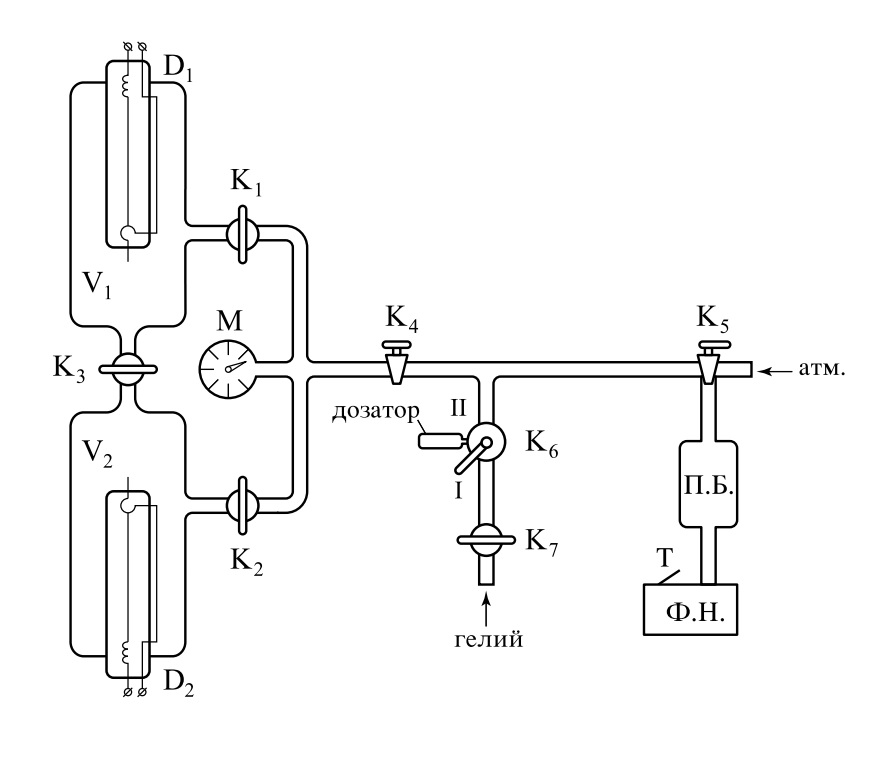
\includegraphics[width=1.00\textwidth]{1.jpg}
	\caption{Установка для определения коэффициента диффузии}
	\label{fig:Установка}
\end{figure}

\subsection{Параметры установки}
{\bf Объём цилиндра для гелия: } $V = 775 \pm 10 $ $cм^3$

{\bf Объём цилиндра для воздуха: } $V = 775 \pm 10 $ $cм^3$

{\bf Давление гелия в рабочей смеси: } $P_{гел} = 0.2 P_{раб} $

{\bf Давление гелия в рабочей смеси: } $P_{гел} = 0.2 P_{раб} $

{\bf Атмосферное давление: } $P_{атм} = 98 \pm 0.1$ КПа $= 980 \pm 1$ КБ

{\bf Характеристика отверстия: } $\frac{l}{s} = 5.3 \pm 0.1 1/см$

\subsection{Инструментальные погрешности}
{\bf Вакуумметр: } $\Delta = \pm 500 $ Па

\section{Результаты измерений и обработка данных}
\subsection{Проверка зависимости разности концентраций}
Убедимся, что процесс диффузии подчиняется закону (\ref{eq:n}).
Для этого для каждого опыта построим графики $\ln V (T)$ на рис. \ref{fig:G41}, \ref{fig:G75}, \ref{fig:G120}, \ref{fig:G150}, \ref{fig:G191}.

\begin{figure}[p]
	\centering
		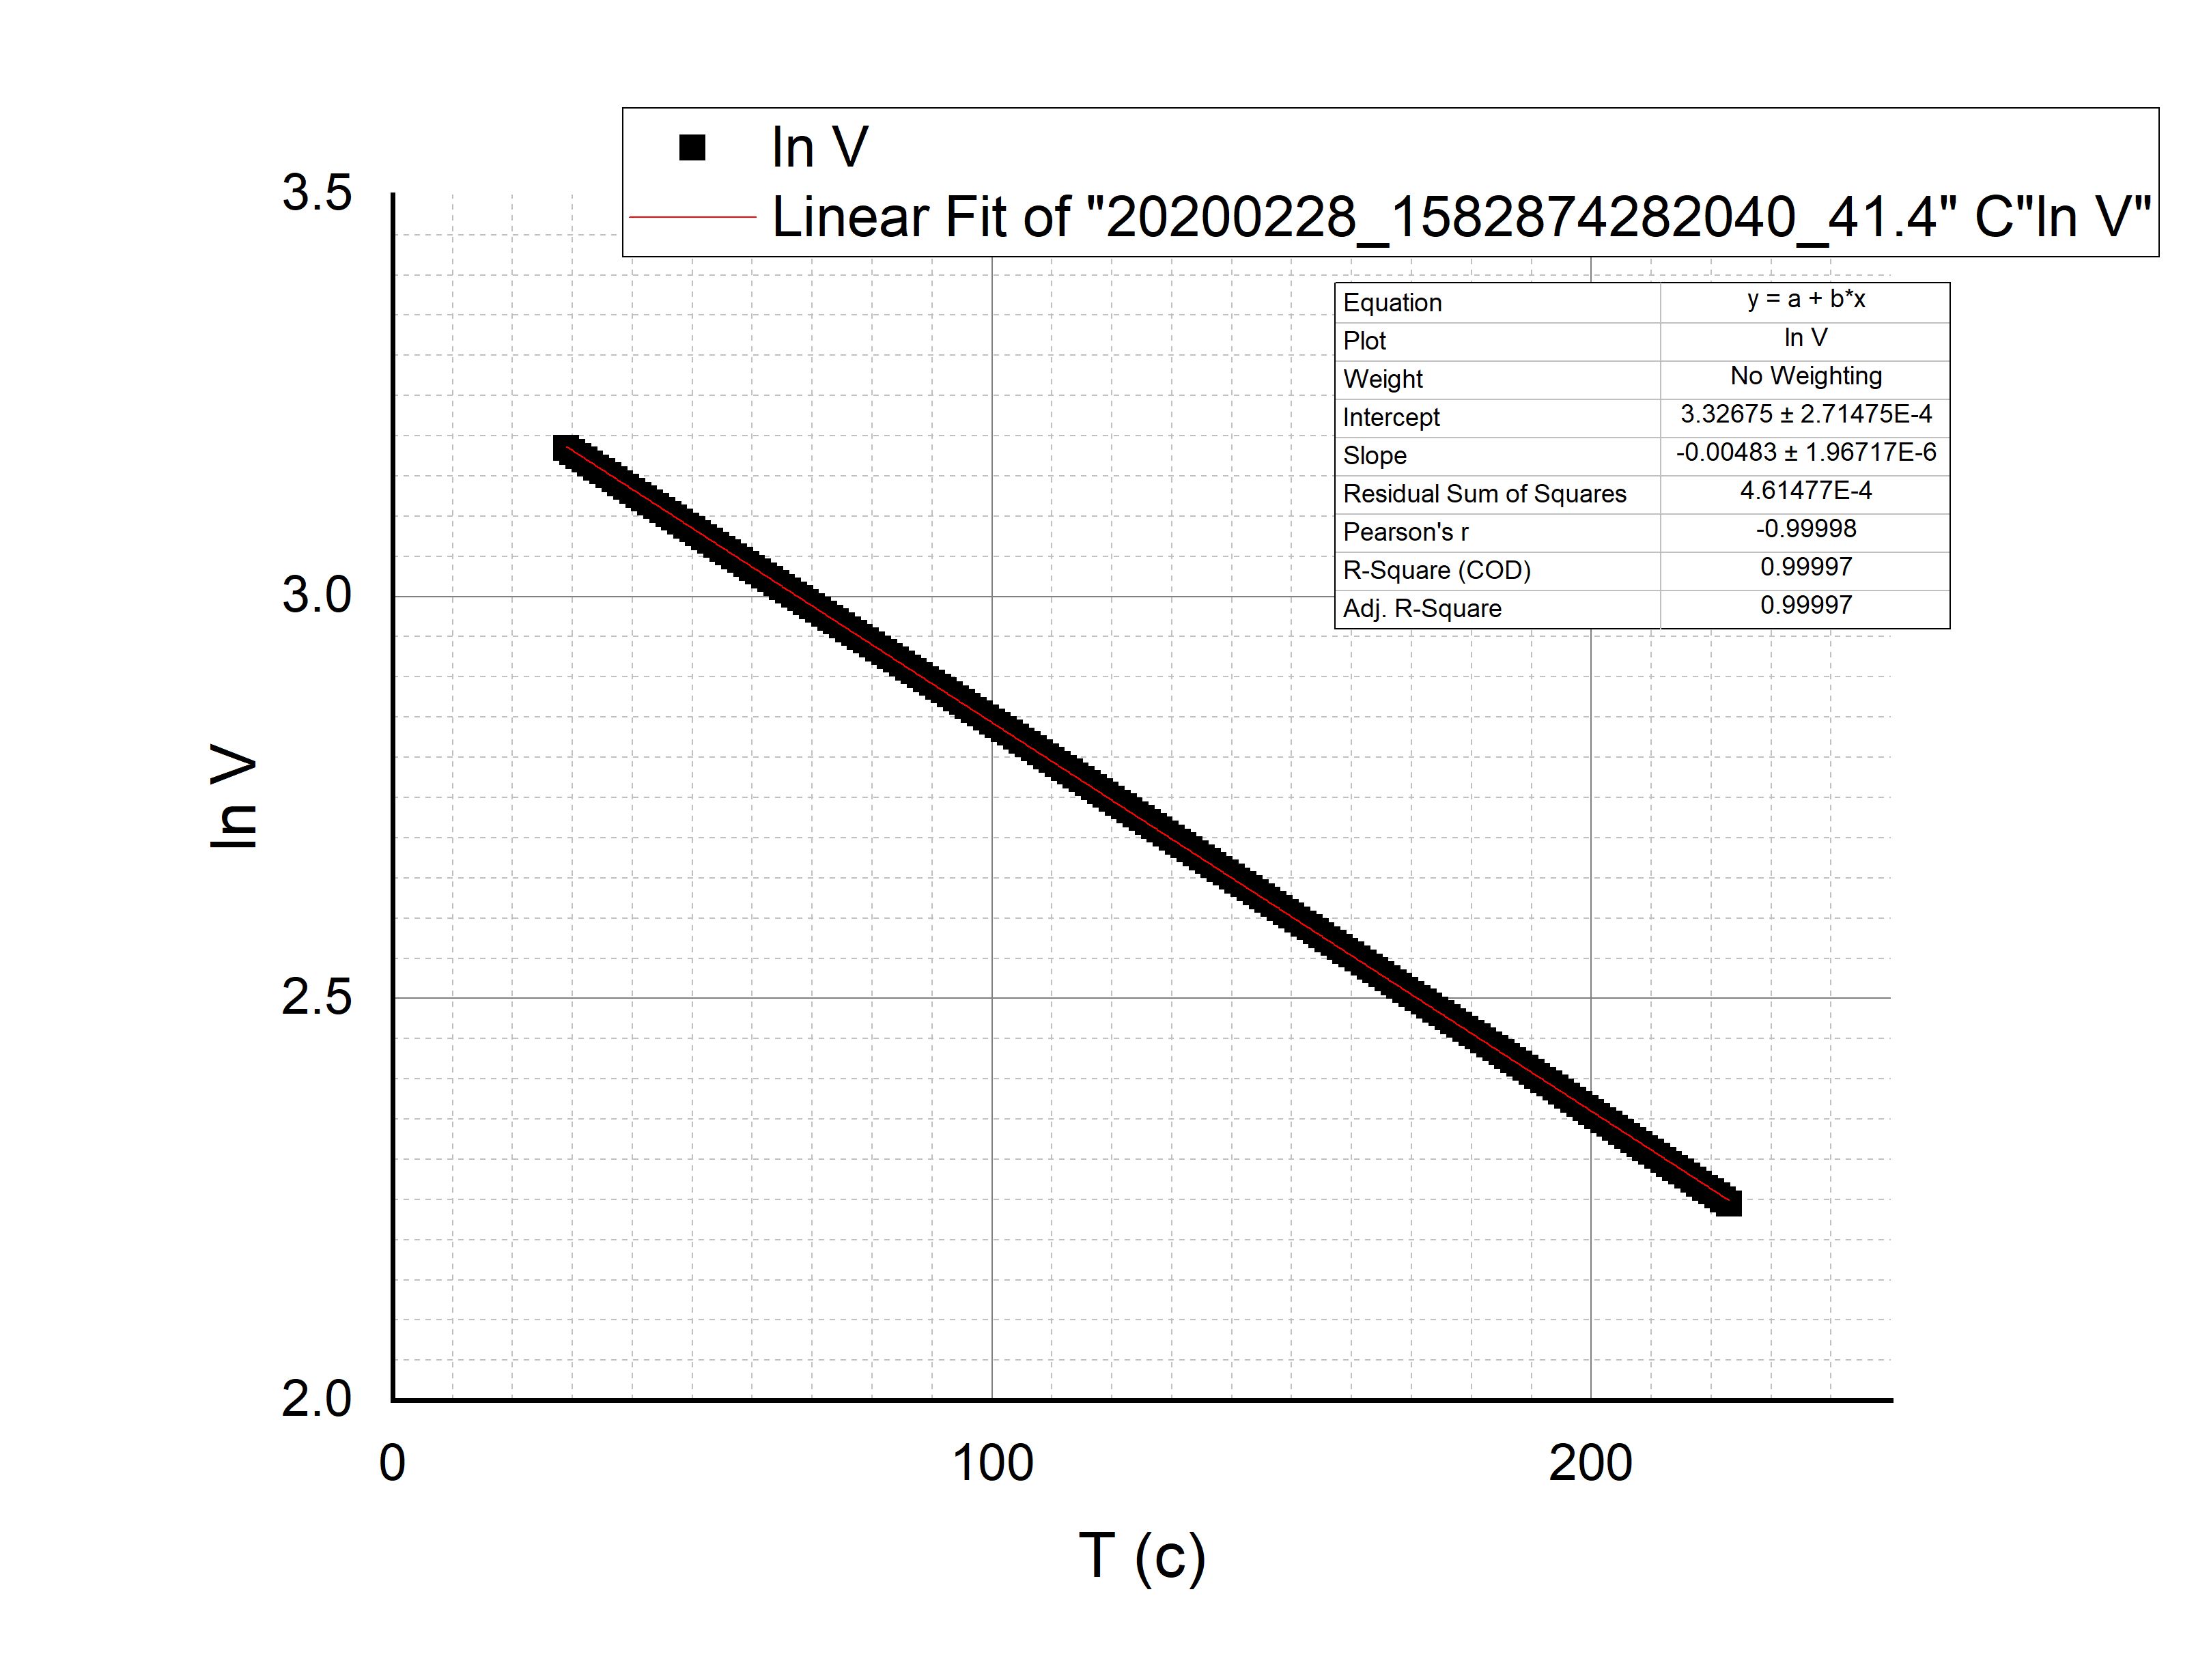
\includegraphics[width=0.75\textwidth]{G41.jpg}
	\caption{График для давления 41 торр}
	\label{fig:G41}
\end{figure}

\begin{figure}[p]
	\centering
		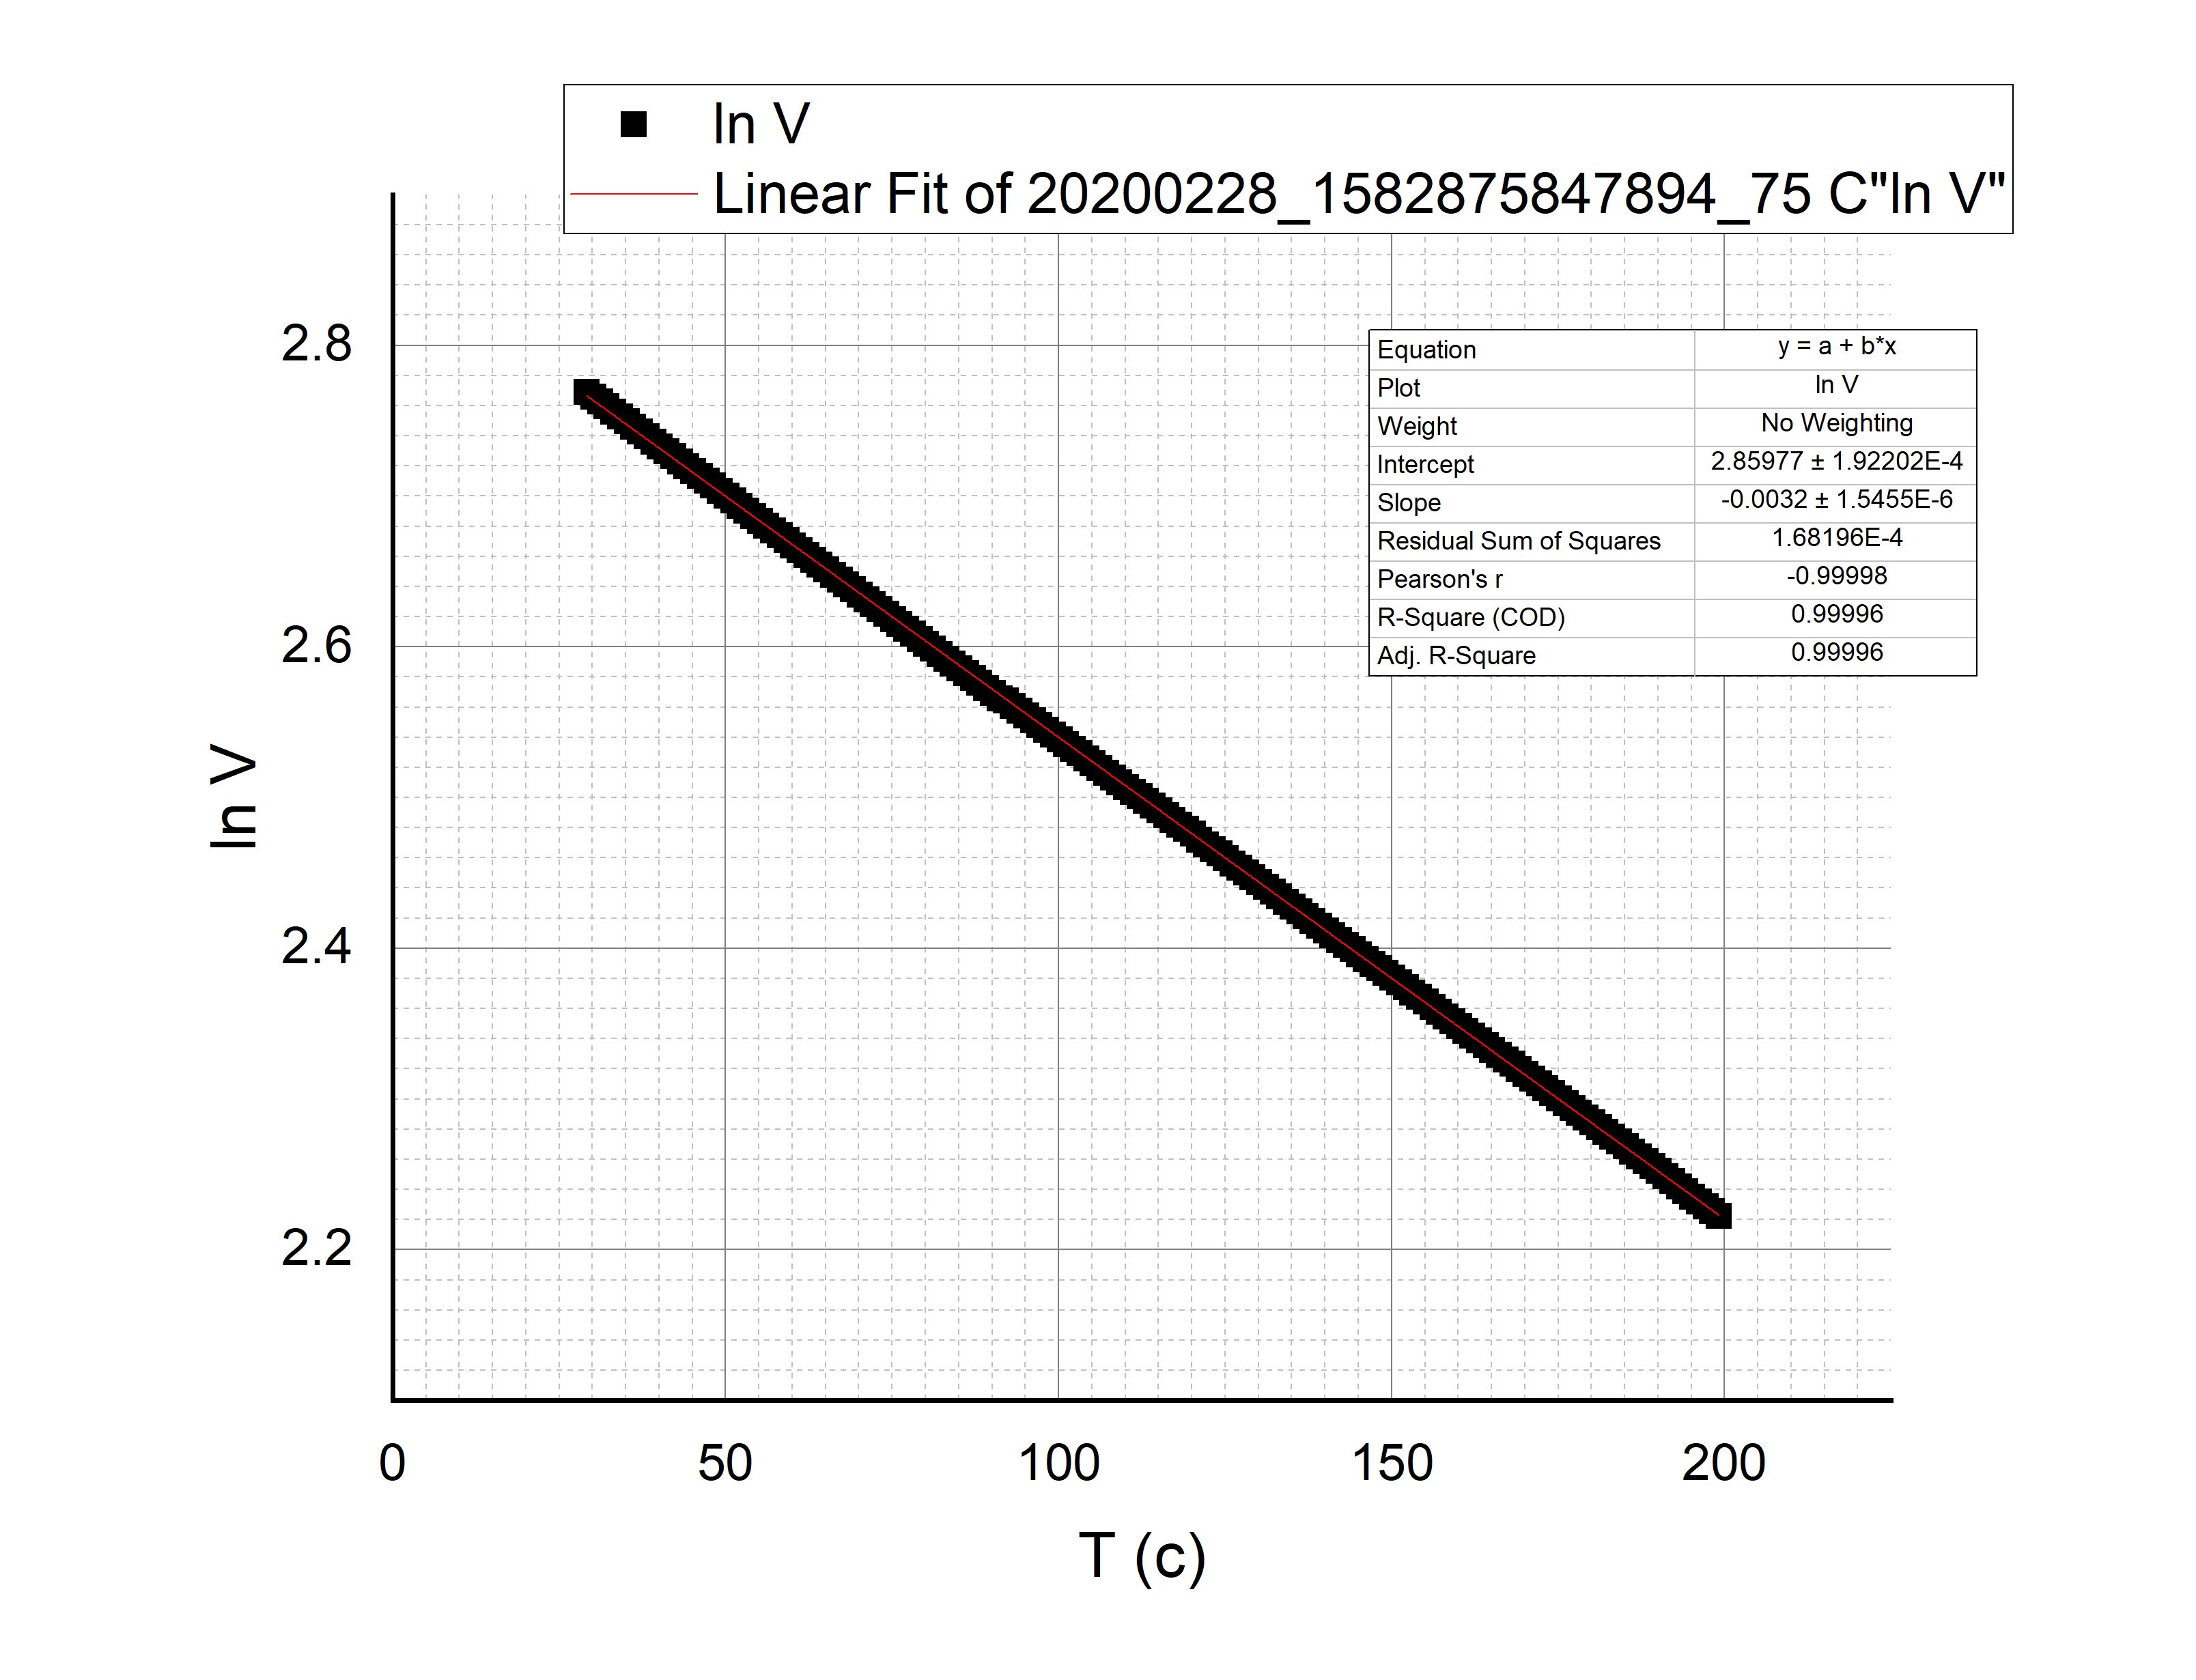
\includegraphics[width=0.75\textwidth]{G75.jpg}
	\caption{График для давления 75 торр}
	\label{fig:G75}
\end{figure}

\begin{figure}[p]
	\centering
		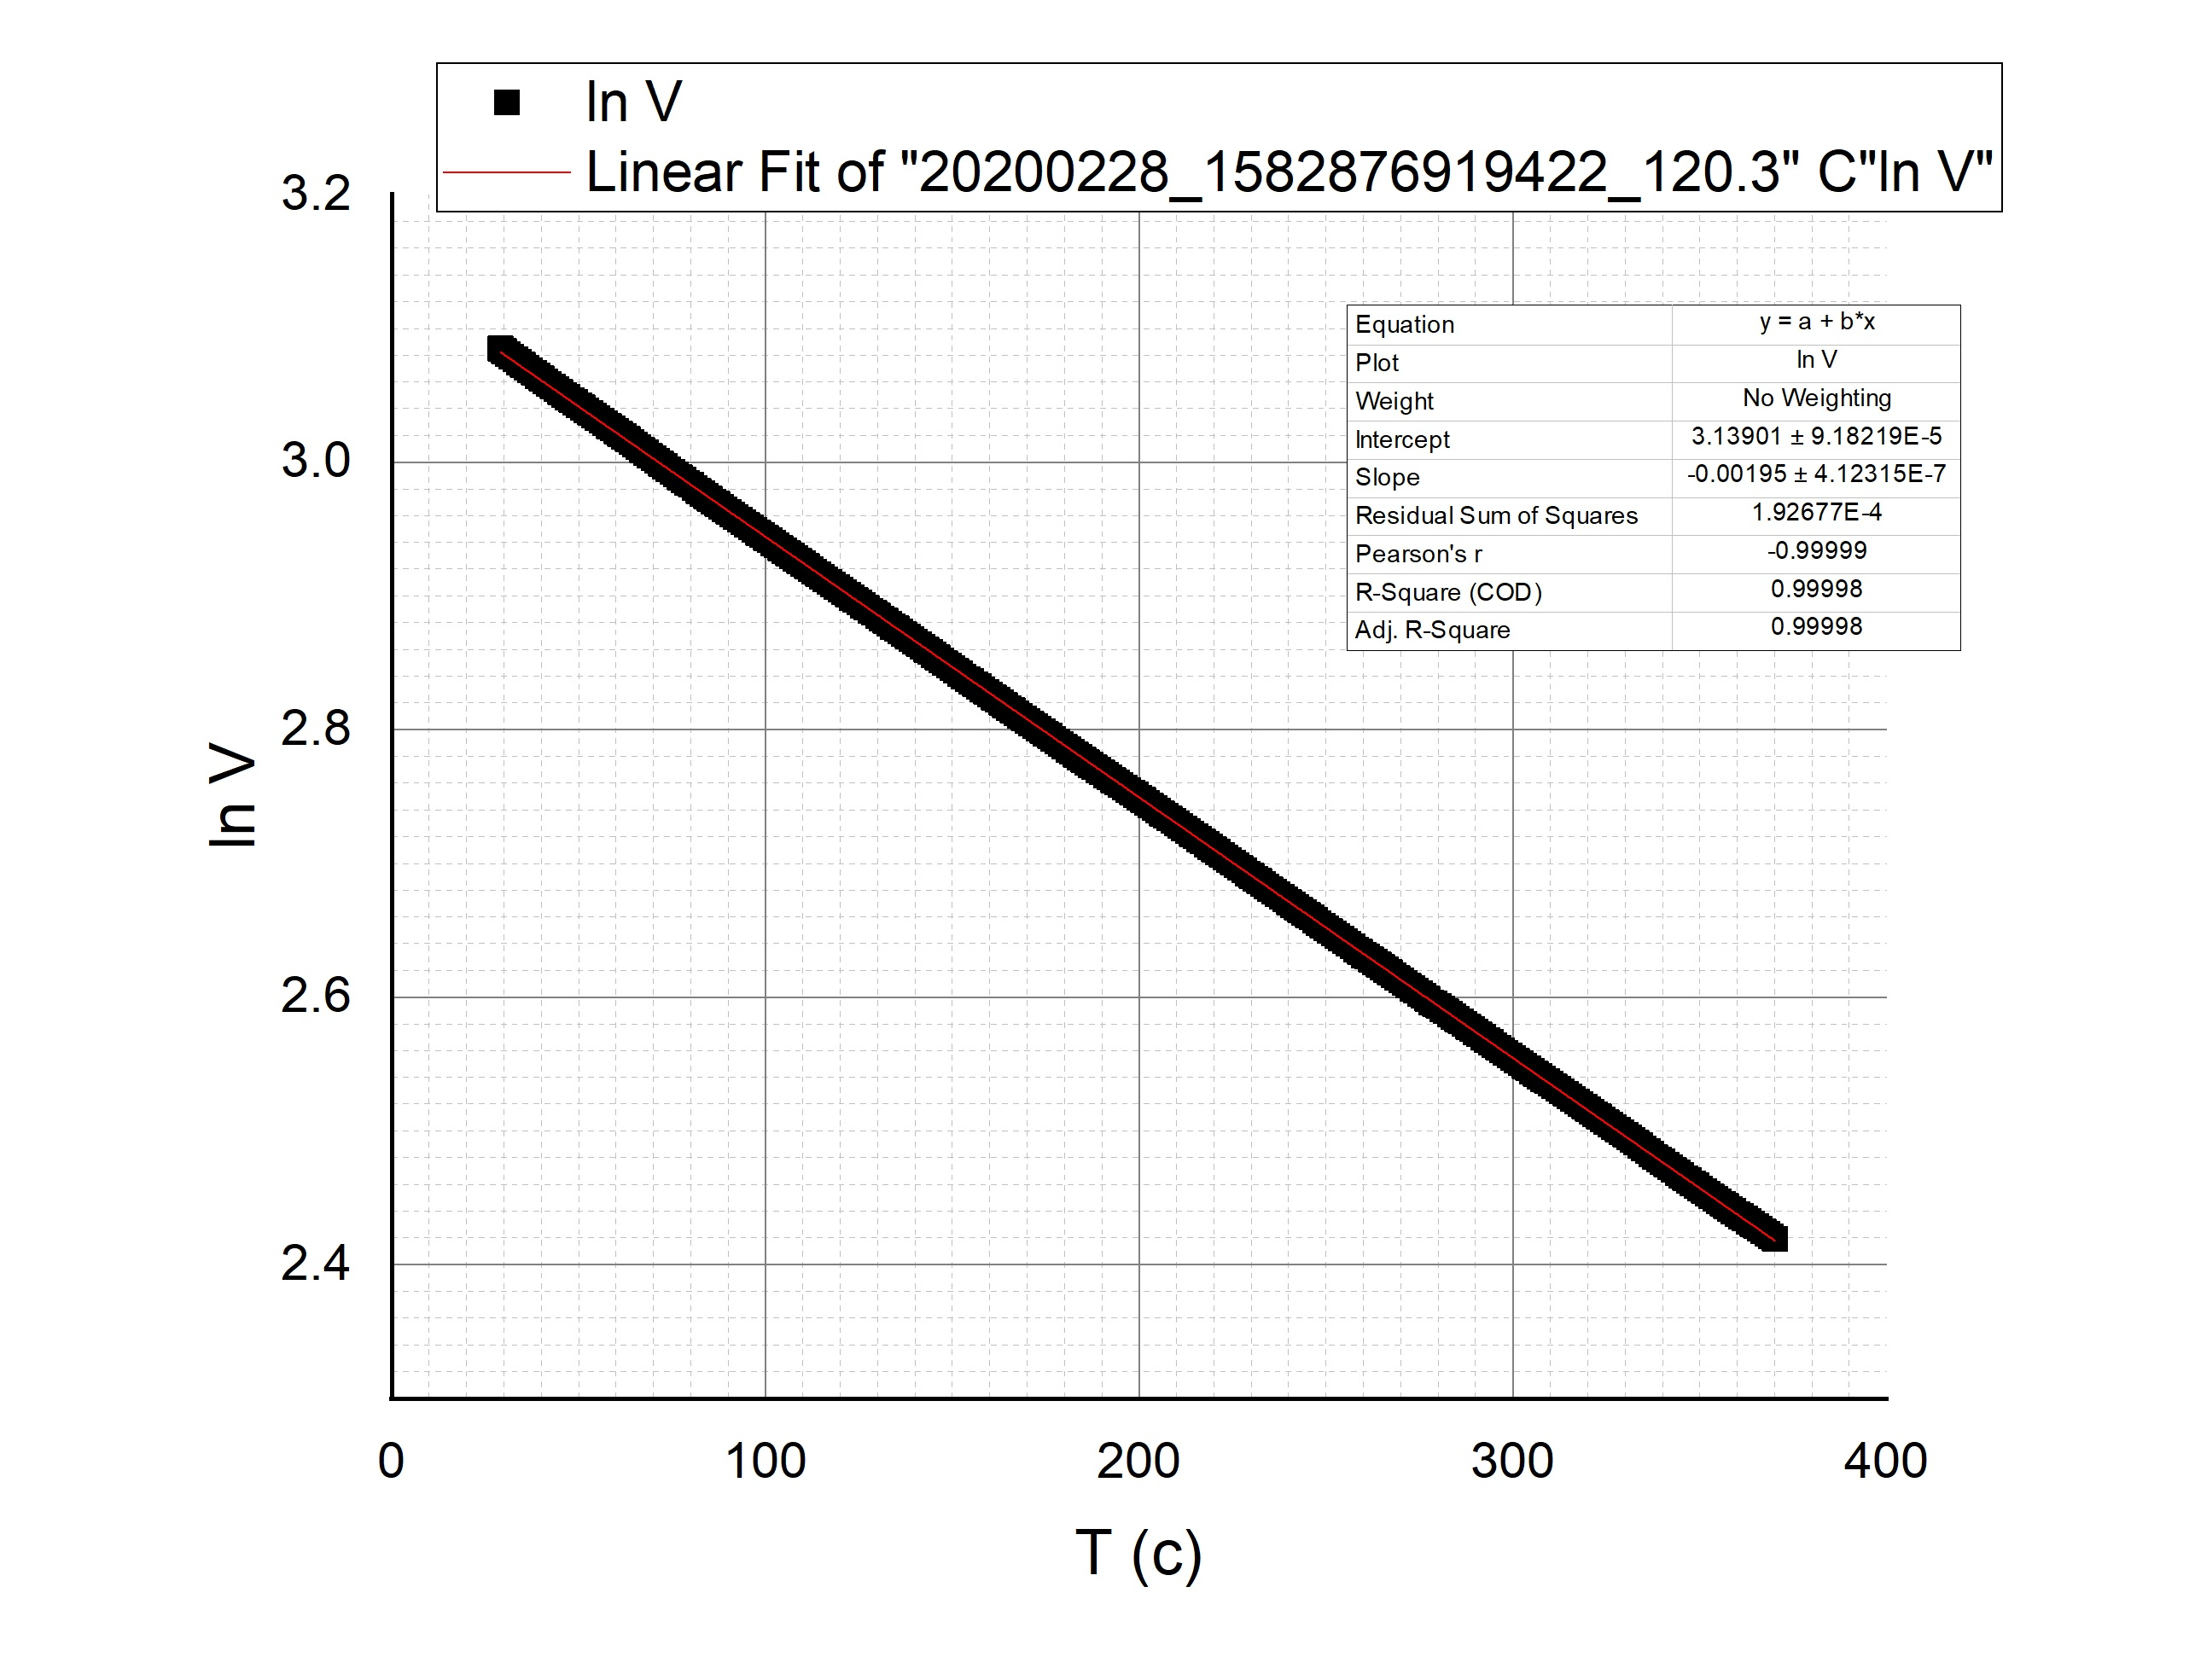
\includegraphics[width=0.75\textwidth]{G120.jpg}
	\caption{График для давления 120 торр}
	\label{fig:G120}
\end{figure}

\begin{figure}[p]
	\centering
		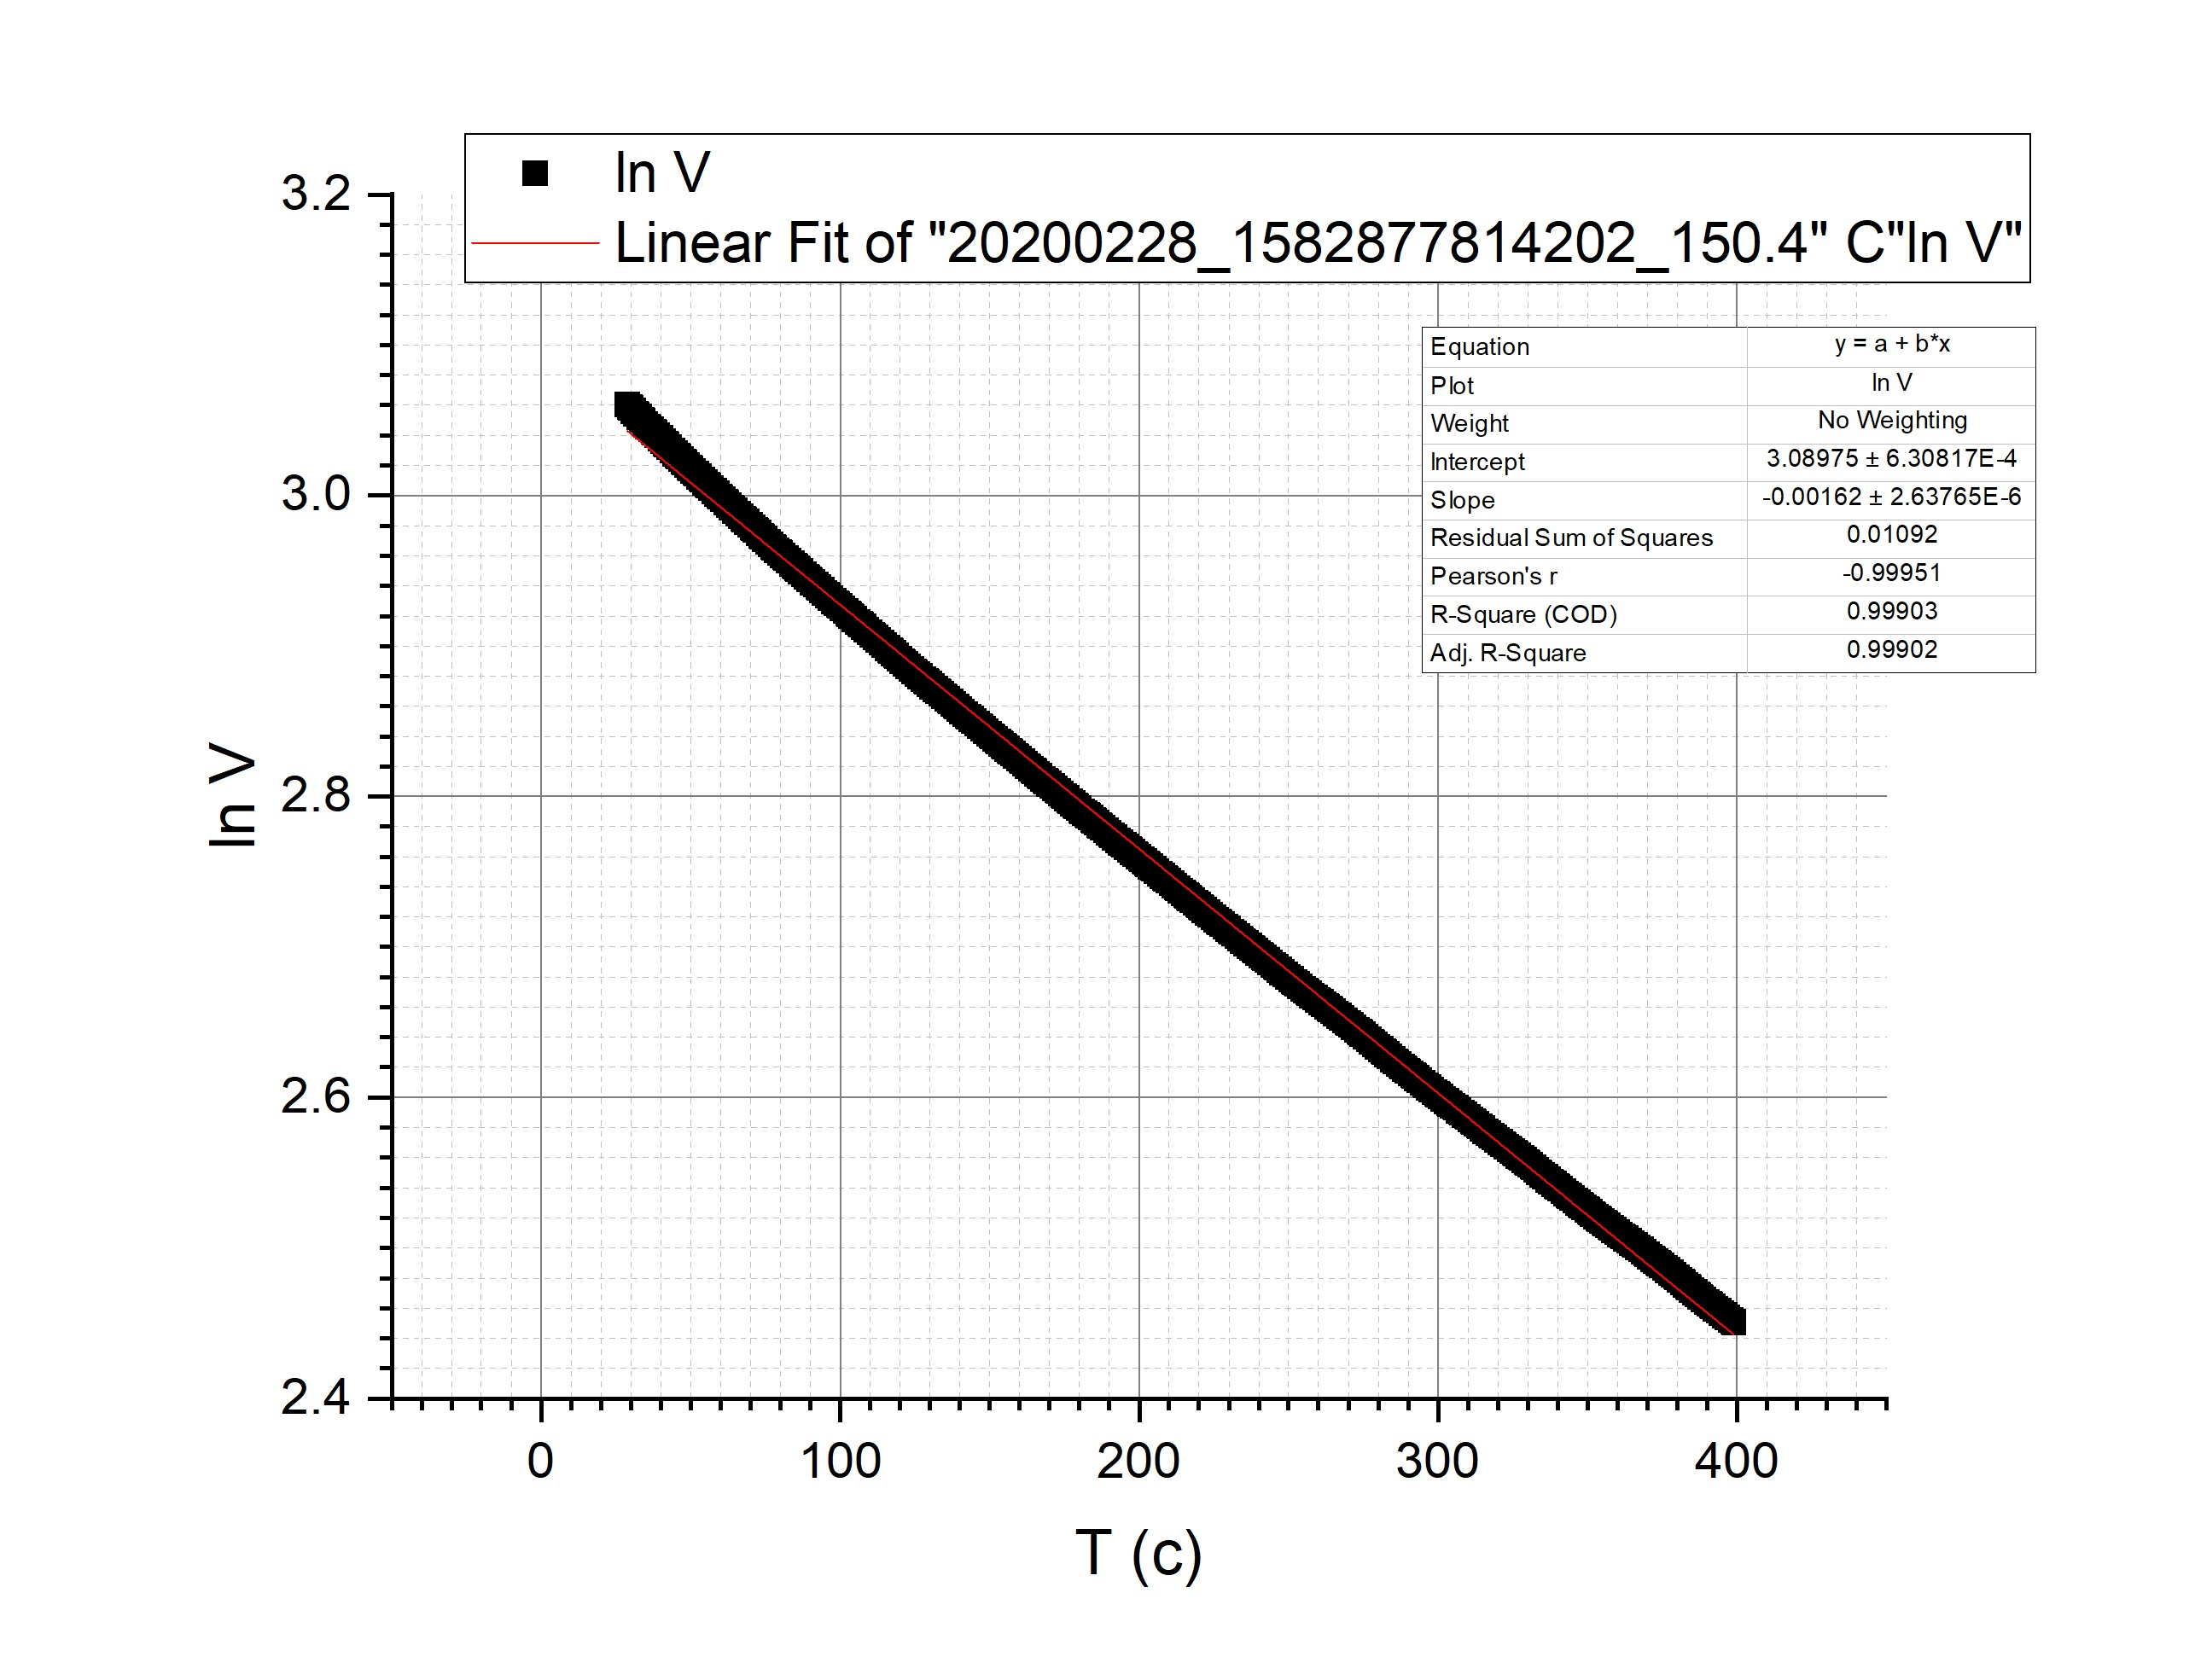
\includegraphics[width=0.75\textwidth]{G150.jpg}
	\caption{График для давления 150 торр}
	\label{fig:G150}
\end{figure}

\begin{figure}[p]
	\centering
		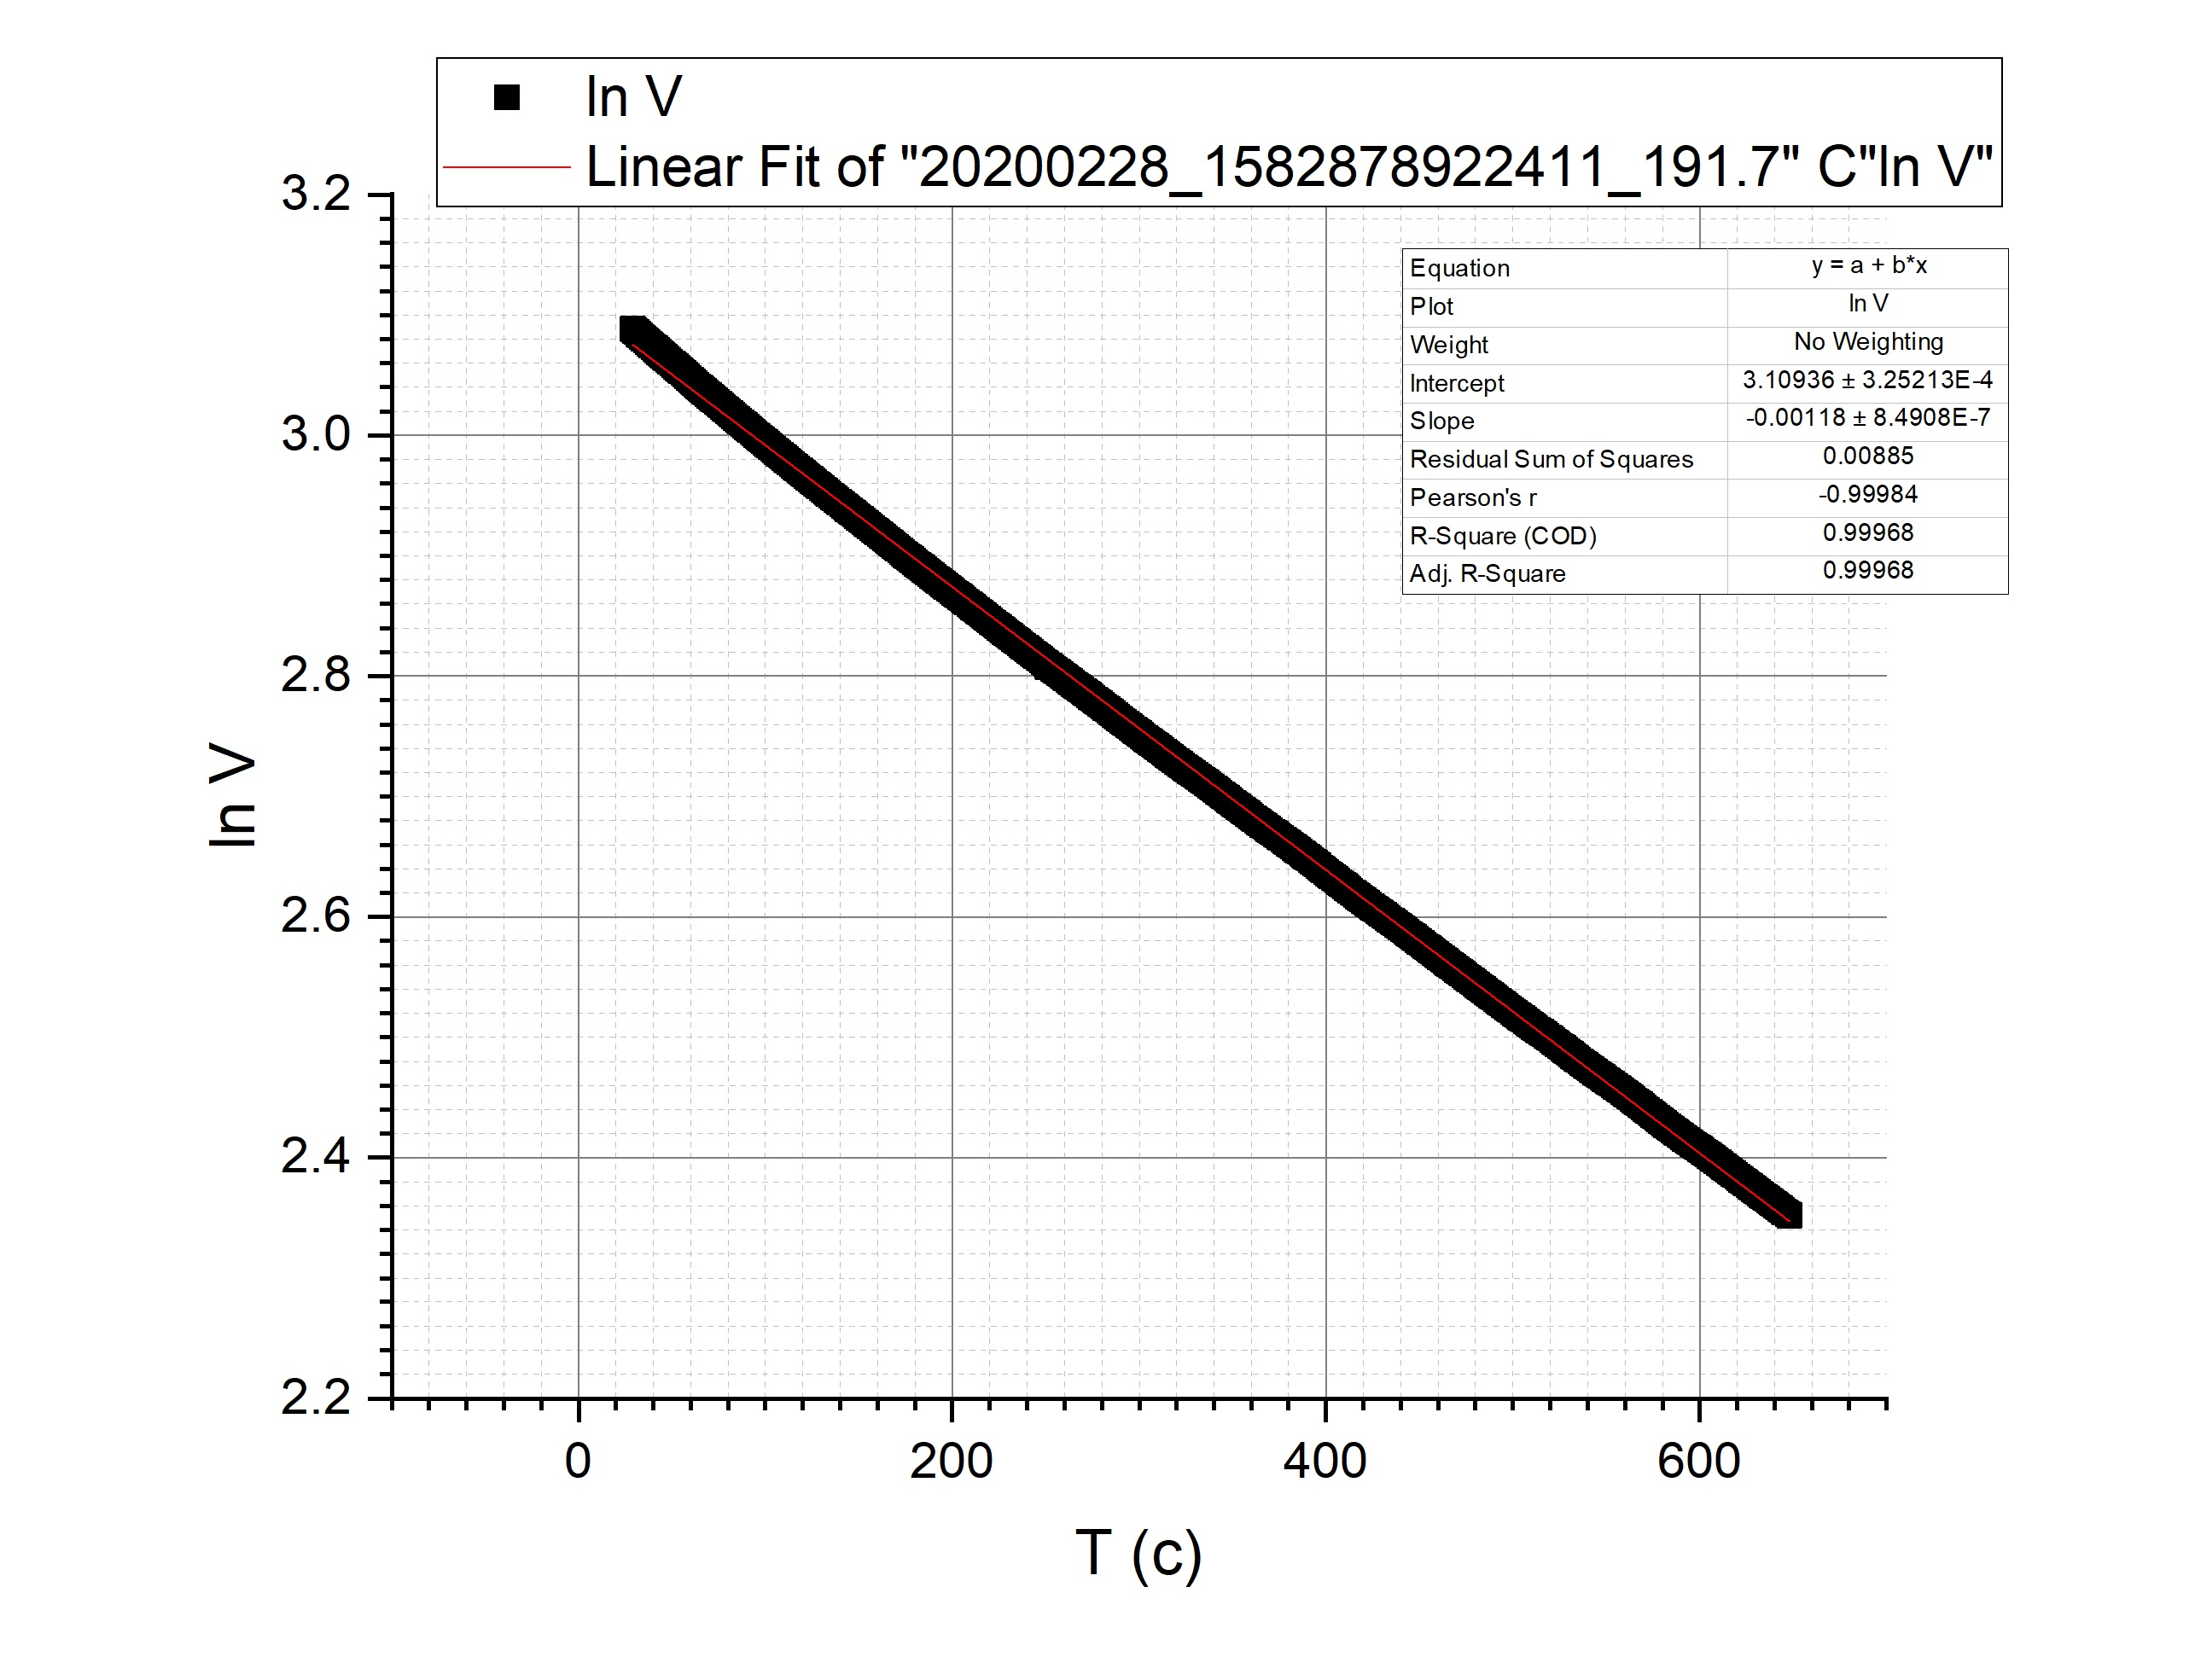
\includegraphics[width=0.75\textwidth]{G191.jpg}
	\caption{График для давления 191 торр}
	\label{fig:G191}
\end{figure}
Вcе графики, кроме \ref{fig:G150} с достаточной точностью являются прямыми линиями.
\subsection{Определение коэффициента диффузии}
Чтобы вычислить $D$ -- коэффициент диффузии, учтём, что $n_1 - n_2 \propto U$ и что $V_1 = V_2$, и преобразуем формулу (\ref{eq:tau}) к виду:
\begin{eqnarray}
D = \frac{l V}{2 \tau S}, \\
D = \frac{l V}{2 (-\frac{1}{k}) S},
\label{eq:Расчётная}
\end{eqnarray}
где $k$ -- тангенс угла наклона графиков.

Расчитаем коэффициент диффузии с учётом погрешностей. Погрешность $D$ вычисляется по формуле 
\begin{equation}
\sigma_D = D \sqrt{\frac{\sigma^{2}_{\frac{l}{s}} S^2}{l^2} + \frac{\sigma^{2}_{V}}{V^2} + \frac{\sigma^{2}_{\tau}}{\tau^2}}
\label{eq:}
\end{equation}

\begin{table}[htbp]
	\centering
		\begin{tabular}{|l|l|l|}
\hline
Давление, Б & k, 1/с   & Коэффициент диффузии D, $\frac{м^2}{с}$ \\ \hline
5.50E+04    & -0.00483 & $9.9 \pm 0.2$                       \\ \hline
1.00E+05    & -0.00320 & $6.6 \pm 0.2$                        \\ \hline
1.60E+05    & -0.00195 & $4.00 \pm 0.09$                         \\ \hline
2.00E+05    & -0.00162 & $3.33 \pm 0.08$                          \\ \hline
2.55E+05    & -0.00118 & $2.42 \pm 0.06$                           \\ \hline
\end{tabular}
	\caption{Коэффициент диффузии при разных давлениях}
	\label{tab:КоэффициентДиффузииПриРазныхДавлениях}
\end{table}
\subsection{Определение среднего пробега молекулы $\lambda$}
Нанесём полученные результаты на график \ref{fig:К.Дифф.}. 
\begin{figure}[htbp]
	\centering
		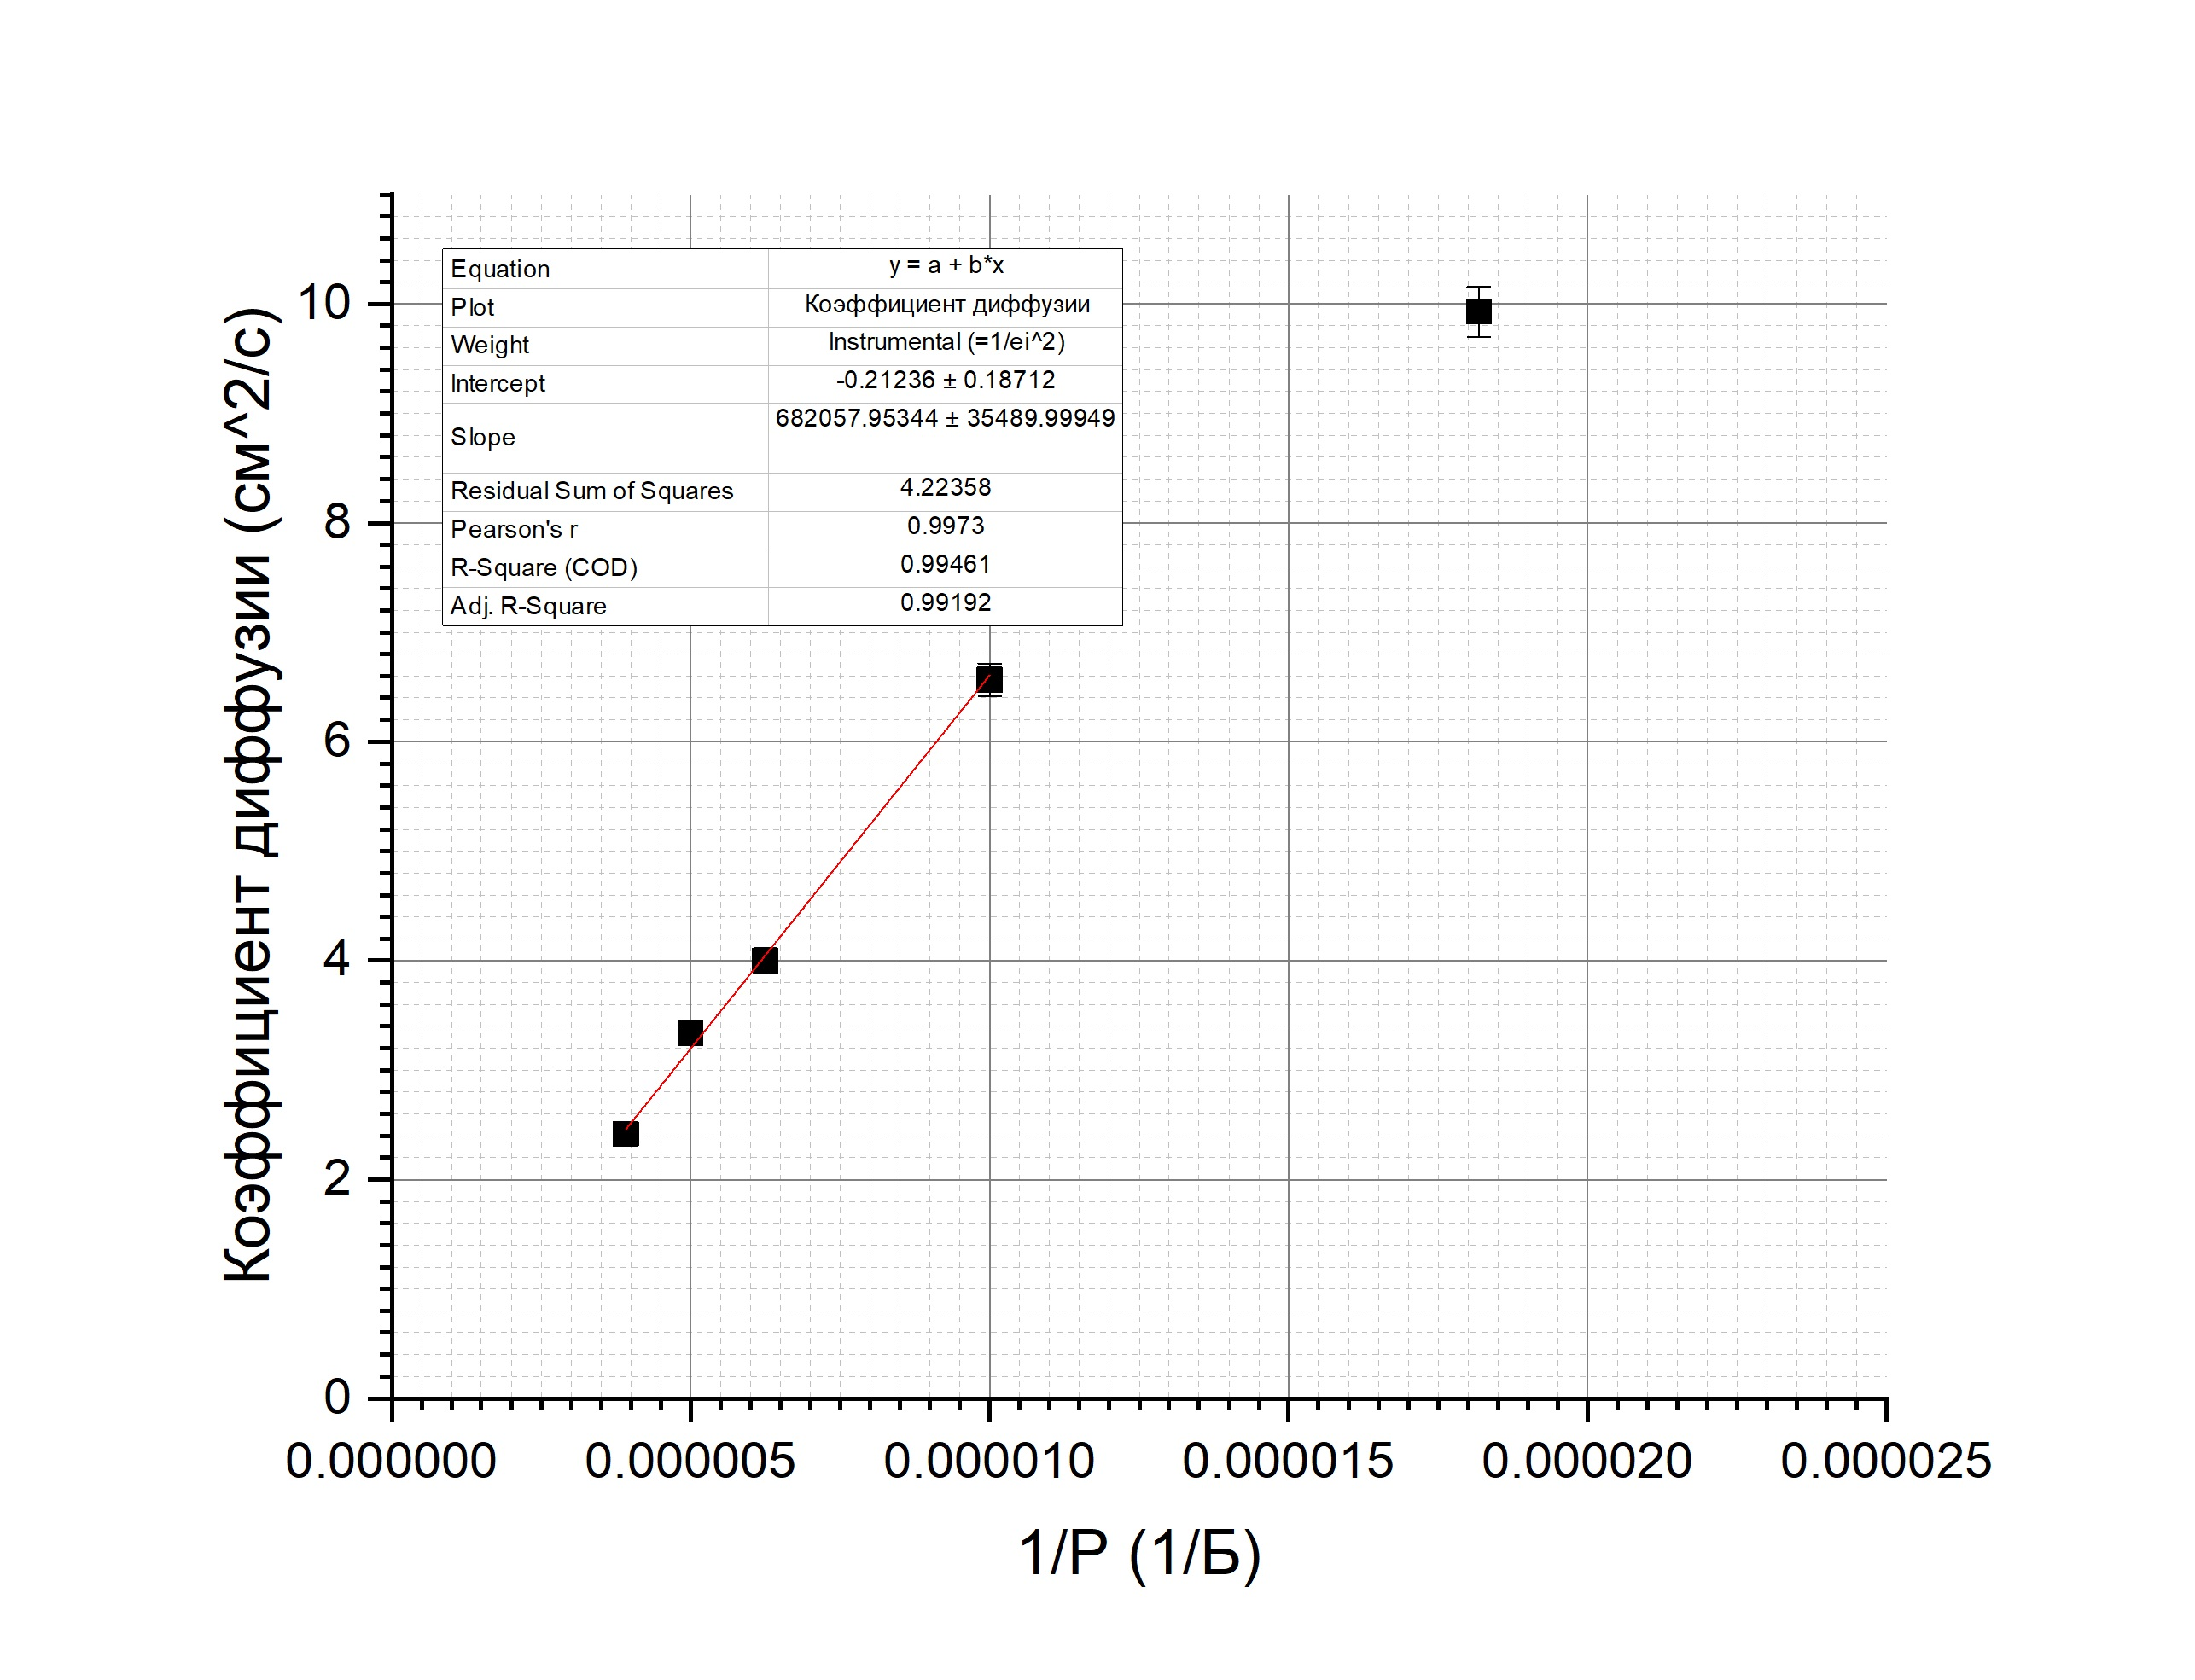
\includegraphics[width=0.75\textwidth]{К. Дифф..jpg}
	\caption{Зависимость $D (\frac{1}{P})$}
	\label{fig:К.Дифф.}
\end{figure}
Точки, отображающие результаты опытов, должны ложиться на прямую, т. к. в формуле (\ref{eq:current}) $J \propto P$. По всей видимости, на опыте при $P = 55000$ Б была допущена ошибка в подготовке рабочей смеси, что привело к неверному результату (см. график \ref{fig:К.Дифф.}). Используем остальные результаты.

Экстраполируем прямую до значения атмосферного давления 1013250 Б. 
\begin{equation}
D = \frac{k}{P} = 0.67 \pm 0.03 \frac{см^2}{с}
\label{eq:экстраполяция}
\end{equation}
Применим формулу (\ref{eq:ДиффузияИПробег}). Тогда $\lambda = 4.35 * 10^{-5}$ см.

По формуле $\lambda = \frac{1}{\sigma n}$, где $n = n_0$ -- число Лошмидта, получим $\sigma = 8.5 * 10^{-16} см^2$
\section{Вывод}
При помощи датчиков теплопроводности определили зависимости концентраций гелия в воздухе от времени при различных давлениях газов; по результатам измерений определили константу диффузии, оценили в условиях опыта длину свободного пробега молекул и эффективную площадь их поперечного сечения
\end{document}

